\documentclass[a4paper,11pt,oneside]{scrartcl}
\parindent 0pt
\usepackage[utf8]{inputenc}
\usepackage[german]{babel}
\usepackage{amsmath}
\usepackage{amssymb}
\usepackage{stmaryrd}
\usepackage{graphicx}

%opening
\title{Digitale Bildverarbeitung - Lösung Blatt 3 (Fourier-Transf., Splines, DFT)}
\author{Thomas Waldecker\\Stefan Giggenbach}

\begin{document}

\maketitle

\newpage

\section*{Aufgabe 1: Fourier-Beziehungen}
\subsection*{1a) Verschiebung im Ortsbereich}

$\mathcal{F}\{f(x-\alpha,y-\beta)\}=\iint_{-\infty}^{\infty}f(x-\alpha,y-\beta)\cdot e^{-j2\pi(xu+yv)} dx dy$ \\

Mit den Substitutionen $\xi=x-\alpha$ ($x=\xi+\alpha$) und $\eta=y-\beta$ ($y=\eta+\beta$) ergibt sich \\

$=\iint_{-\infty}^{\infty}f(\xi,\eta)\cdot e^{-j2\pi((\xi+\alpha)u+(\eta+\beta)v)} d\xi d\eta$ \\

Durch Ausklammern der konstanten Faktoren erhält man \\

$=e^{-j2\pi(\alpha u+\beta v)}\iint_{-\infty}^{\infty}f(\xi,\eta)\cdot e^{-j2\pi(\xi u+\eta v)} d\xi d\eta$ \\

Da das Integral der Fouriertransformation $\mathcal{F}\{f(\xi,\eta)\}=F(u,v)$ entspricht folgt \\

$\mathcal{F}\{f(x-\alpha,y-\beta)\}=F(u,v)\cdot e^{-j2\pi(\alpha u+\beta v)}$

\subsection*{1b) Faltungssatz}

$\mathcal{F}\{h(x,y)\ast f(x,y)\}=\iint_{-\infty}^{\infty}[\iint_{-\infty}^{\infty}h(\chi,\psi)\cdot f(x-\chi,y-\psi) d\chi d\psi]\cdot e^{-j2\pi(xu+yv)} dx dy$ \\

Durch Ausklammern und Umstellen der konstanten Faktoren erhält man \\

$=\iint_{-\infty}^{\infty}h(\chi,\psi)\cdot[\iint_{-\infty}^{\infty}f(x-\chi,y-\psi)\cdot e^{-j2\pi(xu+yv)} dx dy] d\chi d\psi$ \\

Da das innere Integral mit der Beziehung aus Teilaufgabe 1a) der Fouriertransformation $\mathcal{F}\{f(x-\chi,y-\psi)\}=F(u,v)\cdot e^{-j2\pi(\chi u+\psi v)}$ entspricht folgt \\

$=\iint_{-\infty}^{\infty}h(\chi,\psi)\cdot F(u,v)\cdot e^{-j2\pi(\chi u+\psi v)} d\chi d\psi$ \\

Durch Ausklammern des konstanten Faktor erhält man \\

$=F(u,v)\iint_{-\infty}^{\infty}h(\chi,\psi)\cdot e^{-j2\pi(\chi u+\psi v)} d\chi d\psi$ \\

Da das Integral der Fouriertransformation $\mathcal{F}\{h(\chi,\psi)\}=H(u,v)$ entspricht folgt \\

$\mathcal{F}\{h(x,y)\ast f(x,y)\}=F(u,v)\cdot H(u,v)$

\newpage

\section*{Aufgabe 2: Approximation von sinc(x) durch kubischen Spline}
\subsection*{2a) allgemeine Herleitung}
Ansatz und Ableitungen:\\
\begin{equation*}
\begin{array}{ll}
f(x) & = 
 \left\{ 
  \begin{array}{ll}
   f_1(x) = a_1x^3 + b_1x^2 + c_1x + d_1 & \text{für} \quad 0 < x < 1\\
   f_2(x) = a_2x^3 + b_2x^2 + c_2x + d_2 & \text{für} \quad 1 < x < 2\\
   f_3(x) = 0 & \text{sonst}\\
  \end{array} 
 \right.
\\[1cm]
f'(x) & = 
 \left\{ 
  \begin{array}{ll}
   f_1'(x) = 3a_1x^2 + 2b_1x + c_1 & \text{für} \quad 0 < x < 1\\
   f_2'(x) = 3a_2x^2 + 2b_2x + c_2 & \text{für} \quad 1 < x < 2\\
   f_3'(x) = 0 & \text{sonst}\\
  \end{array} 
 \right.
\\[1cm]
f''(x) & = 
 \left\{
  \begin{array}{ll}
   f_1''(x) = 6a_1x + 2b_1 & \text{für} \quad 0 < x < 1\\
   f_2''(x) = 6a_2x + 2b_2 & \text{für} \quad 1 < x < 2\\
   f_3''(x) = 0 & \text{sonst}\\
  \end{array}
 \right.
 \end{array}
\end{equation*}

Einsetzen der bekannten Werte der Funktion und der Ableitung an der Stelle 0 ergibt direkt Lösungen für $c_1$ und $d_1$:
\begin{align*}
&f_1(0) = 1 = a_1 \cdot 0 + b_1 \cdot 0 + c_1 \cdot 0 + d_1 \Rightarrow \underline{d_1 = 1}\\
&f_1'(0) = 0 = 3a_1 \cdot 0 + 2b_1 \cdot 0 + c_1 \Rightarrow \underline{c_1 = 0}
\end{align*}

Durch das Einsetzen der übrigen Funktions- und Ableitungswerte an den jeweiligen Grenzen der Splines ergeben sich fünf Gleichungen:
\begin{align}
f_1(1) = & 0 = a_1 + b_1 + 1\label{g1}\\
f_2(1) = & 0 = a_2 + b_2 + c_2 + d_2\label{g2}\\
f_2(2) = & 0 = 8a_2 + 4b_2 + 2c_2 + d_2\label{g3}\\
f_1'(1) = & f_2'(1): 3a_1 + 2b_1 = 3a_2 + 2b_2 + c_2\label{g4}\\
f_2'(2) = & 0 = 12a_2 + 4b_2 + c_2\label{g5}
\end{align}

Zuerst wird $c_2$ mit Gleichung \eqref{g5} aus $a_2$ und $b_2$ ausgedrückt:
\begin{equation*}12a_2 + 4b_2 + c_2 = 0 \Rightarrow \underline{c_2 = -12a_2 - 4b_2}\end{equation*}

Dann wird $d_2$ mit Gleichung \eqref{g2} und dem Ausdruck von $c_2$ aus Gleichung \eqref{g5} auch durch $a_2$ und $b_2$ ausgedrückt:
\begin{align*}
&a_2 + b_2 + c_2 + d_2 = 0\\
&d_2 = -a_2 - b_2 - c_2\\
&d_2 = -a_2 - b_2 + 12a_2 +4b_2\\
&\underline{d_2 = 11a_2 + 3b_2}
\end{align*}

Mit Gleichung \eqref{g3} und den vorherigen Ausdrücken von $c_2$ und $d_2$ können wir $b_2$ als Funktion von $a_2$ darstellen:
\begin{align*}
&8a_2 + 4b_2 + 2c_2 + d_2 = 0\\
&8a_2 + 4b_2 + 2(-12a_2 - 4b_2) + 11a_2 + 3b_2 = 0\\
&a_2(8-24+11) + b_2(4-8+3) = 0\\
&\underline{b_2 = -5a_2}
\end{align*}

Durch Einsetzen dieses Ergebnisses in die aufgelösten Gleichungen \eqref{g2} und \eqref{g5} können wir dort das $b_2$ eliminieren:
\begin{align*}
&c_2 = -12a_2 - 4b_2\\
&c_2 = -12a_2 -4(-5a_2) = -12a_2 + 20a_2\\
&\underline{c_2 = 8a_2}\\[.3cm]
&d_2 = 11a_2 + 3b_2 = 11a_2 + 3(-5a_2)\\
&\underline{d_2 = -4a_2}
\end{align*}

Mit Gleichung \eqref{g1} wird nun $b_1$ aus $a_1$ ausgedrückt:
\begin{equation*}a_1 + b_1 = -1 \Rightarrow \underline{b_1 = -1 -a_1}\end{equation*}

Dies und die Ergebnisse für $b_2$, $c_2$ und $d_2$ werden nun in Gleichung \eqref{g4} eingesetzt:
\begin{align*}
&3a_1 + 2b_1 = 3a_2 + 2b_2 + c_2\\
&3a_1 + 2(-1 -a_1) = 3a_2 + 2(-5a_2) + 8a_2\\
&a_1 -2 = 3a_2 - 10a_2 + 8a_2\\
&\underline{a_1 = a_2 + 2}
\end{align*}

Das Ergebins in \eqref{g1} eingesetzt ergibt den Ausdruck für $b_1$:
\begin{align*}
&b_1 = -1 - a_1\\
&b_1 = -1 - (a_2 + 2)\\
&\underline{b_1 = -a_2 - 3}
\end{align*}

\subsection*{2b) Lösung im Skript}
\begin{equation*}
s3(t) = 
 \left\{ 
  \begin{array}{ll}
   \lvert t^3\rvert - 2t^2 + 1 & \text{für} \quad 0 \leq t < 1\\
   - \lvert t^3\rvert + 5t^2 -8\rvert t \lvert +4 & \text{für} \quad 1 \leq \rvert t \lvert < 2\\
   0 & \text{sonst}
  \end{array} 
 \right.
\end{equation*}

Für diese Lösung gilt: $a_2 = -1$. Setzt man dieses $a_2$ in die in 2a berechneten allgemeinen Ausdrücke ein erhält man:
\begin{align*}
a_1 &= a_2 + 2 = -1 + 2 = 1\\
b_1 &= -a_2 - 3 = 1 - 3 = -2\\
c_1 &= 0\\
d_1 &= 1\\
a_2 &= -1\\
b_2 &= -5a_2 = -5(-1) = 5\\
c_2 &= 8a_2 = 8(-1) = -8\\
d_2 &= -4a_2 = -4(-1) = 4
\end{align*}
Diese Lösung stimmt mit der Angabe im Skript überein.

\subsection*{2c) Lösung falls $f_1''(1) = f_2''(1)$}
\begin{align*}
&f_1''(1) = f_2''(1)\\
&6a_1 + 2b_1 = 6a_2 + 2b_2\\
&6(a_2 + 2) + 2(-a_2 - 3) = 6a_2 + 2(-5a_2)\\
&6a_2 + 12 -2a_2 -6 = 6a_2 -10a_2\\
&6 = 8a_2\\
&a_2 = \frac{3}{4}
\end{align*}

Die anderen Parameter ergeben sich dann:
\begin{align*}
a_1 &= a_2 + 2 = \frac{3}{4} + 2 = \frac{11}{4}\\
b_1 &= -a_2 - 3 = -\frac{3}{4} - 3 = -\frac{15}{4}\\
c_1 &= 0\\
d_1 &= 1\\
a_2 &= \frac{3}{4}\\
b_2 &= -5a_2 = -5(\frac{3}{4}) = -\frac{15}{4}\\
c_2 &= 8a_2 = 8 \cdot \frac{3}{4} = 12\\
d_2 &= -4a_2 = -4 \cdot \frac{3}{4} = -3
\end{align*}

Interpretation:\\
Wenn die Funktion gezeichnet wird ergibt sich eine Funktion die kein kubischer Spline ist. Es sieht aus als ob bei den Stellen -1 und +1 ein Sprung zwischen den Funktionen vorhanden ist. Dies darf bei Spline-Approximation nicht vorkommen.

\begin{figure}
\begin{center}
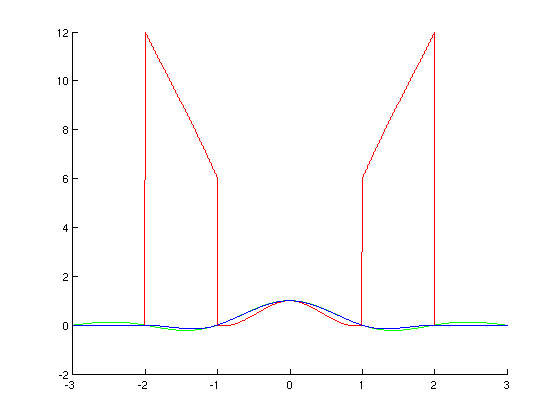
\includegraphics[width=0.5\textwidth]{spline2}
\end{center}
\caption{Die Funktion mit $f_1''(1) = f_2''(1)$ (rot)}
\end{figure}

Rechnerische überprüfung:
\begin{align*}
f_1(1) &= f_2(1)\\
\frac{11}{4}t^3 - \frac{15}{4}t^2 + 1 &= \frac{3}{4}t^3 - \frac{15}{4}t^2 + 12t - 3\\
\frac{11}{4} - \frac{15}{4} + 1 &= \frac{3}{4} - \frac{15}{4} + 12 - 3\\
\frac{11}{4} + 1 - \frac{3}{4}  - 12 + 3 &= 0\\
2+1-12+3&=0\\
-6&=0 \quad \lightning
\end{align*}
Die rechnerische Überprüfung ergibt das die "Lösung" gar keine richtige Lösung des Gleichungssystems ist.
\begin{figure}
\begin{center}
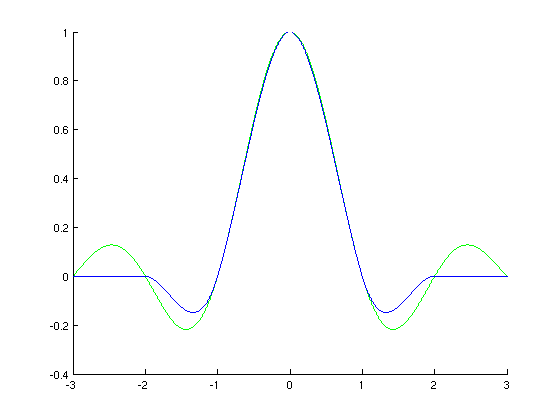
\includegraphics[width=.5\textwidth]{spline1}
\end{center}
\caption{Der kubische Spline (blau) und die sinc(x) Funktion (grün)}
\end{figure}
\newpage

\section*{Aufgabe 3: DFT/Abtastung/Abtasttheorem}
\subsection*{a)}

$\Delta x=\frac{L}{N}=\frac{10\,mm}{256}=0.0391\,mm$

\subsection*{b)}

$u_{a}=\frac{N}{L}=\frac{256}{10\,mm}=25.6\,\frac{1}{mm}$

\subsection*{c)}

$\Delta u=\frac{1}{N\Delta x}=\frac{1}{256\cdot0.0391\,mm}= 0.1\,\frac{1}{mm}$

\subsection*{d)}

Die Schwingung $\sin(16\pi k)$ besitzt eine Kreisfrequenz von $\omega=16\pi\,\frac{1}{mm}$ mit $\omega=2\pi f$ also eine Frequenz von $f=\frac{16\pi}{2\pi}\,\frac{1}{mm}=8\,\frac{1}{mm}$. Zusammen mit dem Intervall $\Delta u$ aus Tailaufgabe c) ergeben sich \\

$l_{1}=\frac{f}{\Delta u}=\frac{8\,\frac{1}{mm}}{0.1\,\frac{1}{mm}}=80$ und $l_{2}=256-80=176$

\subsection*{e)}

$f_{max}=\frac{u_{a}}{2}=12.8\,\frac{1}{mm}$

\end{document}


